%===================================== CHAP 7 =================================

\chapter{Computational Study} \label{chapter_computational_study}


In this chapter, a computational study based on the solution framework outlined in Chapter \ref{chapter_solution_approach} and the experimental setup in Chapter \ref{chapter_experimental_setup} is presented. First, in Section \ref{sec:exact}, the optimal ex-post decisions are presented. Secondly, in Section \ref{sec:inexact}, the performance of each of different solution approaches are presented. Finally, an ex-post analysis of the risk handling constraints are discussed and presented. 

\newpar

The mathematical model is written in the algebraic modelling language Mosel and implemented in FICO\textsuperscript {\textregistered} Xpress Optimization Suite 8.3, using a HP EliteDesk 800 G3 DM 65W computer with Intel\textsuperscript{\textregistered} Core\textsuperscript{\texttrademark} i7-7700 3.6 GHz processor and 32 GB RAM. The operating system in use is Windows 10 Education 64-bit. The input data to the mathematical model is structured and pre-processed in the statistical programming language R. Further, the results obtained from the mathematical model include decisions on selected squad, starting line-up, substitution priority, number of penalized transfers, captain, vice-captain and whether a gamechip is used in a gameweek. These are written to CSV files, which are exported back to R to calculate how many points the team obtained. In the end, these are further exported to Microsoft Excel to make the data more presentable in form of tables and plots. 

\section{Solution With Realized Points}\label{sec:exact}
This section is divided into three parts. First, the initialization of sets and parameters is presented. Following is a discussion of the problem size and the results obtained by the mathematical model using realized points for the 2017/2018 season. Secondly, the solution is more thoroughly examined to discuss whether the decisions are sensible or not. Finally, the solution is compared against the best performing human managers. 


\subsection{Initialization of parameters}    
%DEL1 

Following in Table \ref{tab:initializations_of_sets} and \ref{tab:initialization_of_parameters} are the initialization of parameters and sets used when the mathematical model with realized points is solved. 

\begin{table}[H]
\centering

\begin{tabular}{@{}lll@{}}
\toprule
Set           &   &                                                               \\ \midrule
$\mathcal{T}$ & - & 35 gameweeks.                                             \\
$\mathcal{P}$ & - & 625 players.                                              \\
$\mathcal{C}$ & - & 20 teams.                                                 \\
$\mathcal{L}$ & - & \{1, 2, 3\}, where 1 is first priority. \\
$\mathcal{T}_{FH}$ & - & Gameweek 1 to 21 is in the first half of the season. \\
$\mathcal{T}_{SH}$ & - & Gameweek 22 to 35 is in the second half of the season. \\
\bottomrule
\end{tabular}
\caption{Initialization of sets.}
\label{tab:initializations_of_sets}
\end{table}

\begin{table}[H] 
\tabcolsep=0.11cm
\centering
\begin{tabular}{@{}lll@{}}
\toprule
Parameters                       &   &                                                                                                \\ \midrule
$\mathlarger{\rho_{pt}}$ & - & Realized points for a player $p$ in a gameweek $t$. \\
$\epsilon$                       & - & Set to 0.1.                                                                     \\
$\kappa_{1}, \kappa_{2}, \kappa_{3} $                     & - & Set to 0.01, 0.001 and 0.0001 respectively.                                               \\
$C_{pt}^{B}$                     & - & Buy price collected from FPL homepage.  \\ 
$R$                              & - & 4 points deducted if number of free transfers is exceeded.       \\
$M^{K}$                          & - &  2 goalkeepers required in the selected squad.                                      \\
$M^{D}$                          & - &  5 defenders required in the selected squad.                         \\
$M^{M}$                          & - & 5 midfielders required in the selected squad.                                     \\
$M^{F}$                          & - & 3 forwards required in the selected squad.                                    \\
$M^{C}$                          & - & 3 players allowed to have from the same team.                                \\
$E$                              & - & 11 players required in the starting line-up.                              \\
$E^{K}$                          & - & 1 goalkeepers required in the starting line-up.                                       \\
$E^{D}$                          & - & 3 defenders required in the starting line-up.                  \\
$E^{M}$                          & - & 3 midfielders required in the starting line-up.                                 \\
$E^{F}$                          & - & 1 forward required in the starting line-up.                     \\
$B^{S}$                          & - & 100 million as starting budget.                                                                              \\
$\beta$                          & - & Set to 1.                                                                                  \\          
$\bar{\alpha}$                   & - & Set to 14.                                                                      \\

$\phi$                           & - & 3 players are substitutes.                                                         \\
$\phi^{K}$                       & - & 1 keeper among the substitutes.                                                          \\
$\overline{Q}$                   & - & 2 free transfers possible to accumulate over gameweeks.                                              \\
$\underline{Q}$                  & - & 1 free transfer given every gameweek.                                      \\ \bottomrule
\end{tabular}
\caption{Initialization of parameters.}
\label{tab:initialization_of_parameters}
\end{table}

 
A season in FPL consists of 38 gameweeks, however because of restriction on time, an early decision was made to solve the model for the first 35 gameweeks. The season is divided in two halves, where the first half is from gameweek 1-21 and the second part is from gameweek 22-35. The transfer window closed after gameweek 26. Until then, 625 players had appeared in at least on game. Thus, the set consists of 625 players.

\newpar

All the parameters specifically stated in the rules of FPL are set accordingly. These include number of points deducted if the number of free transfers are surpassed, number of players in different position in both selected squad and starting line-up, maximum players from same team, starting budget and the restrictions on free transfers. The parameter in the objective function for vice-captain are set to 0.1, while for the substitution priority, $\kappa_{1}, \kappa_{2}, \kappa_{3}$ are set to 0.01, 0.001 and 0.0001, respectively. To tighten the formulation as much as possible, the parameters $\beta$ and $\alpha$ are set so to the smallest, but sufficiently high, value. $\beta$ is used in constraints \eqref{eq:subst} and \eqref{eq:free_hit_subst} in Chapter \ref{chapter_model_formulation} which concern the substitution priority. Considering that the variables adopted are binary, setting the value to 1 is optimal. $\alpha$ is used in constraints \eqref{eq:trans_flow_illegal_transfers}, and is set to highest possible value for number of points-deducting transfers. As 1 free transfer is given each gameweek and the selected squad consists of 15 players, it is not possible to have more than 14 points-deducting transfers. Hence, the parameter $\alpha$ is set accordingly. 



\subsection{Problem Size}

Table \ref{tab:computational_statistics} displays the problem size of FPLDP with input data from the 2017/2018 season. The problem size are given before and after the function Presolve. This is a function integrated in Xpress Optimizer where its objectives are to reduce redundant variables, eliminate redundant constraints and remove linearly dependent constraints, which consequently reduces the complexity of the problem and improve the computing time. As can be seen from the Table \ref{tab:computational_statistics}, the problem size is huge since the number of both constraints and variables are immense. From the table, it can be observed that the Presolve function is successful in eliminating both variables and elements, but the reduction of constraints is not that severe. A reason for this could be that most of the constraints are linearly independent, and that there is a limited presence of empty rows in the FPLDP. In addition, a large part of the $x_{pt}$, $x_{pt}^{freehit}$ and $y_{pt}$ are redundant, as many of them are defined despite few of them are used in the starting line-up and selected squad constraints. The fact that Presolve manages to eliminate such a large number of variables, implies that there should have been used more time and effort on reducing redundant variables in the procedure of implementation. That would most likely have had the effect of reducing solution time. Nonetheless, it can be argued that since the model only has to be solved once, this can to a certain degree be disregarded. 


\begin{table}[H]
\centering
\begin{tabular}{@{}lll@{}}
\toprule
                            & Rows(Constraints)    & Columns(Variables) 
                            \\ \midrule
Original Problem Statistics & 172 034 & 254 425   \\
Xpress Presolve Statistics  & 170 750 & 206 689   \\ 
\bottomrule
\end{tabular}
\caption{Problem size of the model run with realized points.}
\label{tab:computational_statistics}
\end{table}


\subsection{Results of running the model with realized points}

Running the FPLDP with realized points over 35 gameweeks is a big and complex problem, and assuming to obtain optimal solution in reasonable time is a naive assumption. We decided to set the maximum running time to 86 400 seconds, or 1 day. Longer maximum running time than this seems unreasonable. 

\newpar

\begin{figure}[H]
\centering
\begin{minipage}{.5\textwidth}
  \centering
  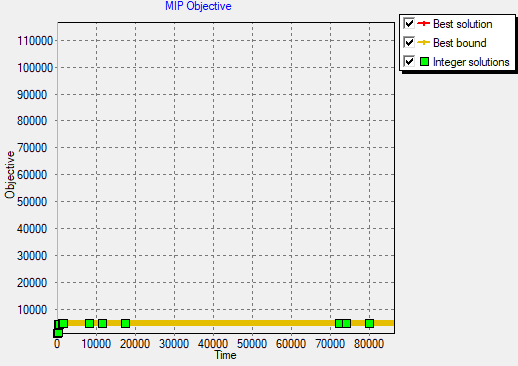
\includegraphics[width=.4\linewidth]{fig/chapter_7/solution_edit_found.png}
  \captionof{figure}{A figure}
  \label{fig:solution_found}
\end{minipage}%
\begin{minipage}{.5\textwidth}
  \centering
  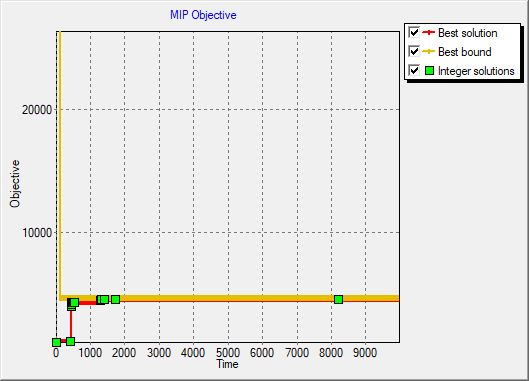
\includegraphics[width=.4\linewidth]{fig/chapter_7/solution_found_edit_zoom_1.png}
  \captionof{figure}{Another figure}
  \label{fig:solution_found_zoom}
\end{minipage}
\end{figure}

\begin{table}[H]
\centering
\begin{tabular}{@{}ll@{}}
\toprule
         &           \\ 
\midrule
Solution & 4553.0302 \\
Gap      & 0.75 \%   \\ 
\bottomrule
\end{tabular}
\caption{Results of the model run with realized points for 2017/2018 season.}
\label{tab:results_realized_points}
\end{table}


The results are given in Table \ref{tab:results_realized_points}. This the best solution found after running the model for 86 400 seconds. The optimal solution was not found in that time, but it is not far off. With a optimality gap of 0.75 \%, the solution is still much better than the best manager and hence regarded as sufficient. It is important to note that the objective value given in
Table \ref{tab:results_realized_points} is from the model run, and hence not directly transferable to total points obtained in FPL. Next, the results from realized points will be discussed into more depth. 



\subsection{Performance in Fantasy Premier League}
In the following we provide the results for the model introduced in chapter \ref{chapter_model_formulation} when solved with realized points, i.e. with perfect information. Figure \ref{Figure_Realized_points} gives an overview of how many points the model obtained in each gameweek. The coloured dots represents gameweeks where the gamechips were used. 

\begin{figure}[H]
\label{fig:Realized_points}
    \centering
    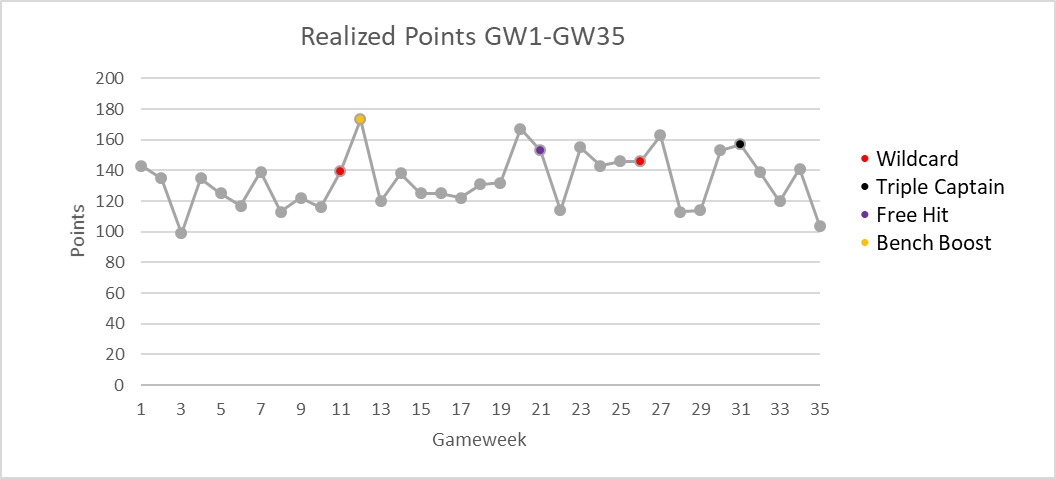
\includegraphics[scale=0.75]{fig/chapter_7/RealizedPoints_colour.png}
    \caption{The graph shows the points per gameweek with perfect information}
\label{Figure_Realized_points}    
\end{figure}

\begin{comment}
We find it necessary to comment on the choices made for selecting when to play the gamechips.
\end{comment}
As observed, the first Wildcard was used one week ahead of the Bench Boost was played. This is reasonable as it is wisely to ensure that you select 15 players that will earn lots of points when playing the Bench Boost. Further, the Free Hit chip was used in gameweek 21, which was a blank gameweek containing only 9 fixtures. It is reasonable to assume that the Free Hit should either be used ahead of a blank or ahead of a double gameweek in order to ensure that all your selected players are featured at least once for that particular gameweek. Finally, the Triple Captain chip was used in gameweek 31 which is reasonable as Mohammed Salah scored 4 goals and had 1 assist in this particular gameweek, yielding a score of 29 points. This was the highest score obtained in one gameweek by any Premier League players. As for the second Wildcard, there is no obvious reason why it was played in gameweek 26, except the fact that it was optimal for the entire solution. 
\newpar
Figure \ref{Figure_Transfers} shows how many transfers the model made ahead of each gameweek. It is notable that the model performs most transfers when the Wildcards and the Free Hit were played. This makes sense as these chips allows you to perform unlimited free transfers. In general, one can say that the model makes many transfers compared to human managers. However, this is due to the fact that this is an optimal solution. Thus, it selects the players that over-performed in a particular gameweek. Every gameweek there are some players that surprise the FPL managers. For instance, if a defender suddenly scores two goals in a match, the goals themselves yield 12 points. 

\begin{figure}[H]
\label{fig_Transfers}
    \centering
    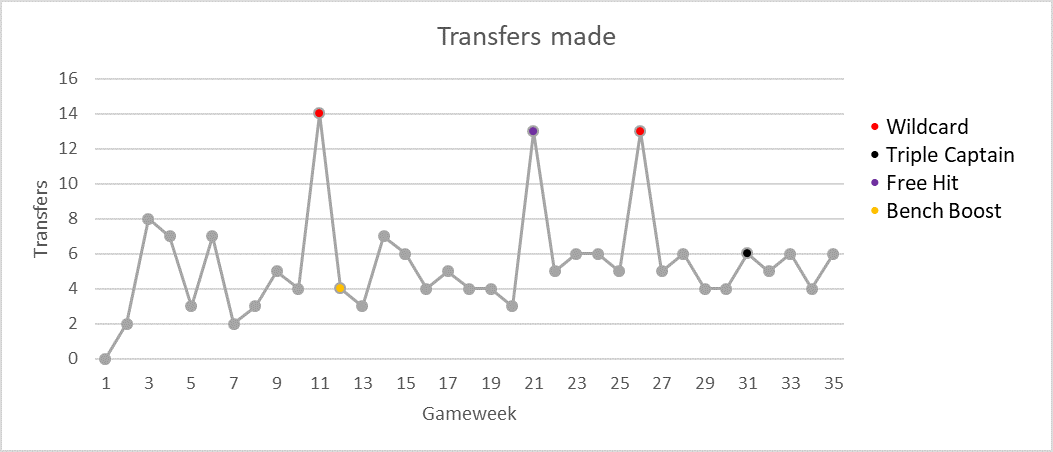
\includegraphics[scale=0.75]{fig/chapter_7/Transfers_colour.png}
    \caption{The graph shows how many transfers the optimal solution makes in every gameweek}
\label{Figure_Transfers}    
\end{figure}

Some readers may find value in comparing the optimal FPL solution to the performance of human managers. Figure \ref{Figure_Comparison} provides a weekly comparison of the weekly average score and the maximum score obtained by human managers to the optimal solution.

\begin{figure}[H]
\label{fig:Comparison}
    \centering
    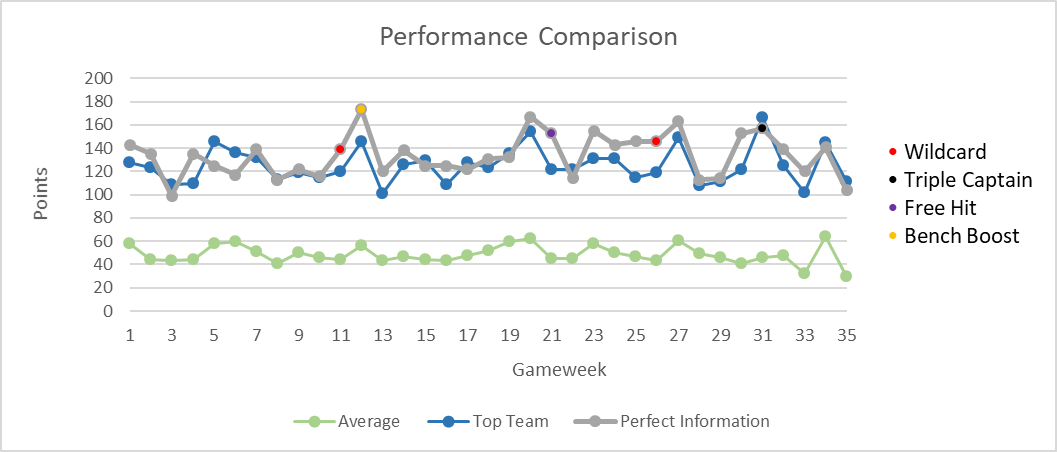
\includegraphics[scale=0.75]{fig/chapter_7/Comparison_colour.png}
    \caption{The graph compares the weekly average and the top performer of each Gameweek to the optimal team with perfect information}
\label{Figure_Comparison}    
\end{figure}

 It is notable that the optimal solution performs well ahead of the weekly average managers, scoring at least twice as many points in every gameweek. Further, it is worth noticing that the optimal overall solution may be beaten by the best manager in individual gameweeks. This is due to the fact that the optimal solution maximizes the points over the entire season, and not only over one particular gameweek. Further, managers that finish top of the gameweek often use a gamechip in order to maximize their weekly score. 
\newpar
There seem to be some positive correlation between the optimal solution and both the weekly top performers as well as the weekly average scores. From table \ref{Figure_Comparison} one can see that the weekly average and the optimal solution have a tendency of moving in the same direction. Hence, when the optimal solution receive a high score, the weekly average have a tendency of doing the same. This might be due to highly selected players performing well in those particular gameweeks. For instance, if a player that has performed well over the entire season receives an abnormal high score during a gameweek, it is anticipated that the weekly average will increase as most managers select this player. Consider Mohamed Salah, who has had an incredible season. At some point he was selected by more than 63\% of the human managers. Thus, when he performs well it is reasonable to assume that both the average and the optimal solution earn numerous points. 
\newpar
As stated in chapter \ref{introduction} it is interesting to compare the optimal solution strategy to that of the manager of leads the overall ranking. Figure \ref{Top_Manager} provides a weekly overview of this comparison.

\begin{figure}[H]
\label{fig:Top_Manager}
    \centering
    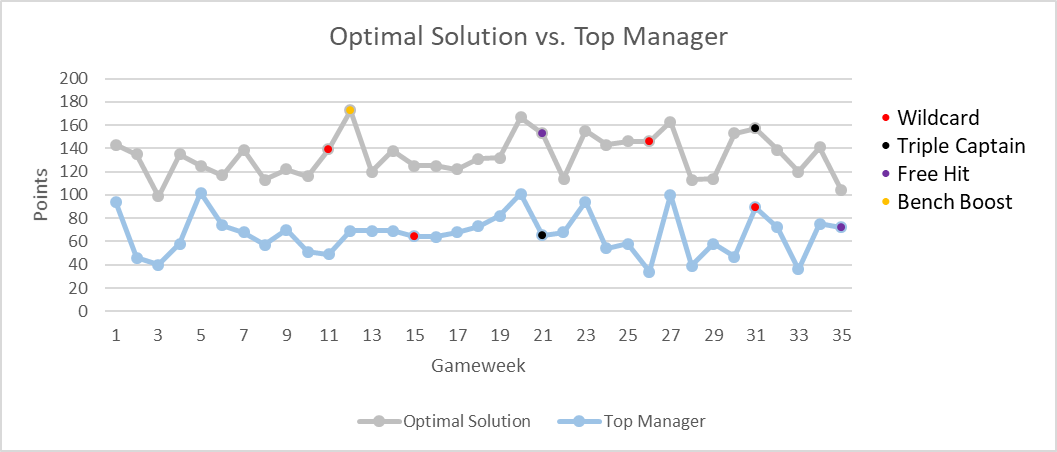
\includegraphics[scale=0.75]{fig/chapter_7/Optimal_vs_Top_colour.png}
    \caption{Comparing optimal solution strategy to top manger}
\label{Top_Manager}    
\end{figure}

As suggested in the introduction, the optimal solution strategy largely outperforms that of the top manager of Fantasy Premier League. In total, it separates 2348 points between the two solutions, more than twice the amount of points gained by the top rated manager. It is notable that the two teams do not play their gamechips in any of the same gameweeks. The top manager played his Triple Captain in gameweek 22, where Tottenham and West Ham were featured twice. Selecting Harry Kane as his Triple Captain is an understandable choice, as Harry Kane was the top scorer of Premier League at that point of time. However, Kane under-performed in both matches only receiving three points in total. In addition, one can see that the top manager played his second Wildcard in gameweek 32, two weeks ahead of a double gameweek. Finally, he played his Free Hit in gameweek 35 which is reasonable as this was ahead of a blank gameweek. As expected, the two teams presented in figure \ref{Top_Manager} are positively correlated.   
\newpar
An other interesting comparison is that of the optimal solution to other human managers. Table \ref{Optimal_Human} provides an overview of how the optimal solution strategy performs compared to the top 50\% of the managers. 

\begin{table}[H]
\centering
\caption{Comparing human managers to optimal solution}
\label{Optimal_Human}
\begin{tabular}{llc}
\hline
                 & Mean   & \multicolumn{1}{l}{Percentage of optimal solution} \\
\hline                 
Optimal solution & 133.63 & 100.00 \%                                          \\
Winner           & 66.54  & 49.80 \%                                           \\
Top 5 \%         & 55.83  & 41.78 \%                                           \\
Top 10 \%        & 54.30  & 40.64 \%                                           \\
Top 20 \%        & 52.20  & 39.06 \%                                           \\
Top 30 \%        & 50.40  & 37.72 \%                                           \\
Top 40 \%        & 48.50  & 36.29 \%                                           \\
Top 50 \%        & 46.50  & 34.80 \%                                           \\
\hline
\end{tabular}
\end{table}

As observed, it is an enormous difference between the optimal solution strategy and that of the other human managers. It is remarkable that the difference in mean between the top 50\% and the winner is only slightly above 20 points per round, while the difference between the optimal solution and the winner is above 67 points. Further, it is notable that the difference between finishing in the top 10 percentile to the top 5 percentile is rather low as it only separates 1.43 points per gameweek. In comparison, the difference between the winner and the 5th percentile is as much as 10.71 points per gameweek. Moreover, an interesting point is that this difference is actually larger than the one between the 50th percentile and the 5th percentile. Hence, it provides reason to assume that in order to finish among the absolute best managers, one have to perform extremely well compared to others. 
\newpar
 


\section{Forecast-based solutions}\label{sec:inexact}

\begin{comment}
\begin{enumerate}
    \item all the gamechips are explained before this chapter. the implementation of the gamechips do not change in each forecasting method. 
    \item a parameter study on the average method for horizon, penalty and obj.value on average forecasts on season 2016. This has been done before computational study. Suggestion figure: matrix for horizon and penalty, with green = good obj value, red = bad obj value
    \item  the decision on the threshold(risk) is explained in Experimental setup method. 
\end{enumerate}
\end{comment}


In this section, we present the computational results for the three different forecasting methods. First, we present and discuss the performance when gamechips are disregarded. Then, we compare the performance of each method when gamechips are included. In order to evaluate the results, we compare the results with the performance of the solution with realized points, the best overall manager and the weekly average among all players. In general, it is important to note that no robust statements can be made due to the lack of available data. However, some insightful observations can be made.

\newpage

\subsection{Results Disregarding Gamechips}

In Figure \ref{fig:res_comp_dis_gamechips} the points obtained by the different forecasting methods are plotted for each gameweek. In Table \ref{tab:res_dis_gamechips}, summarizes the results. Notice that for the Odds method we have presented results for 31 gameweeks, as we only had data for these gameweeks.

\begin{figure}[H]
    \centering
    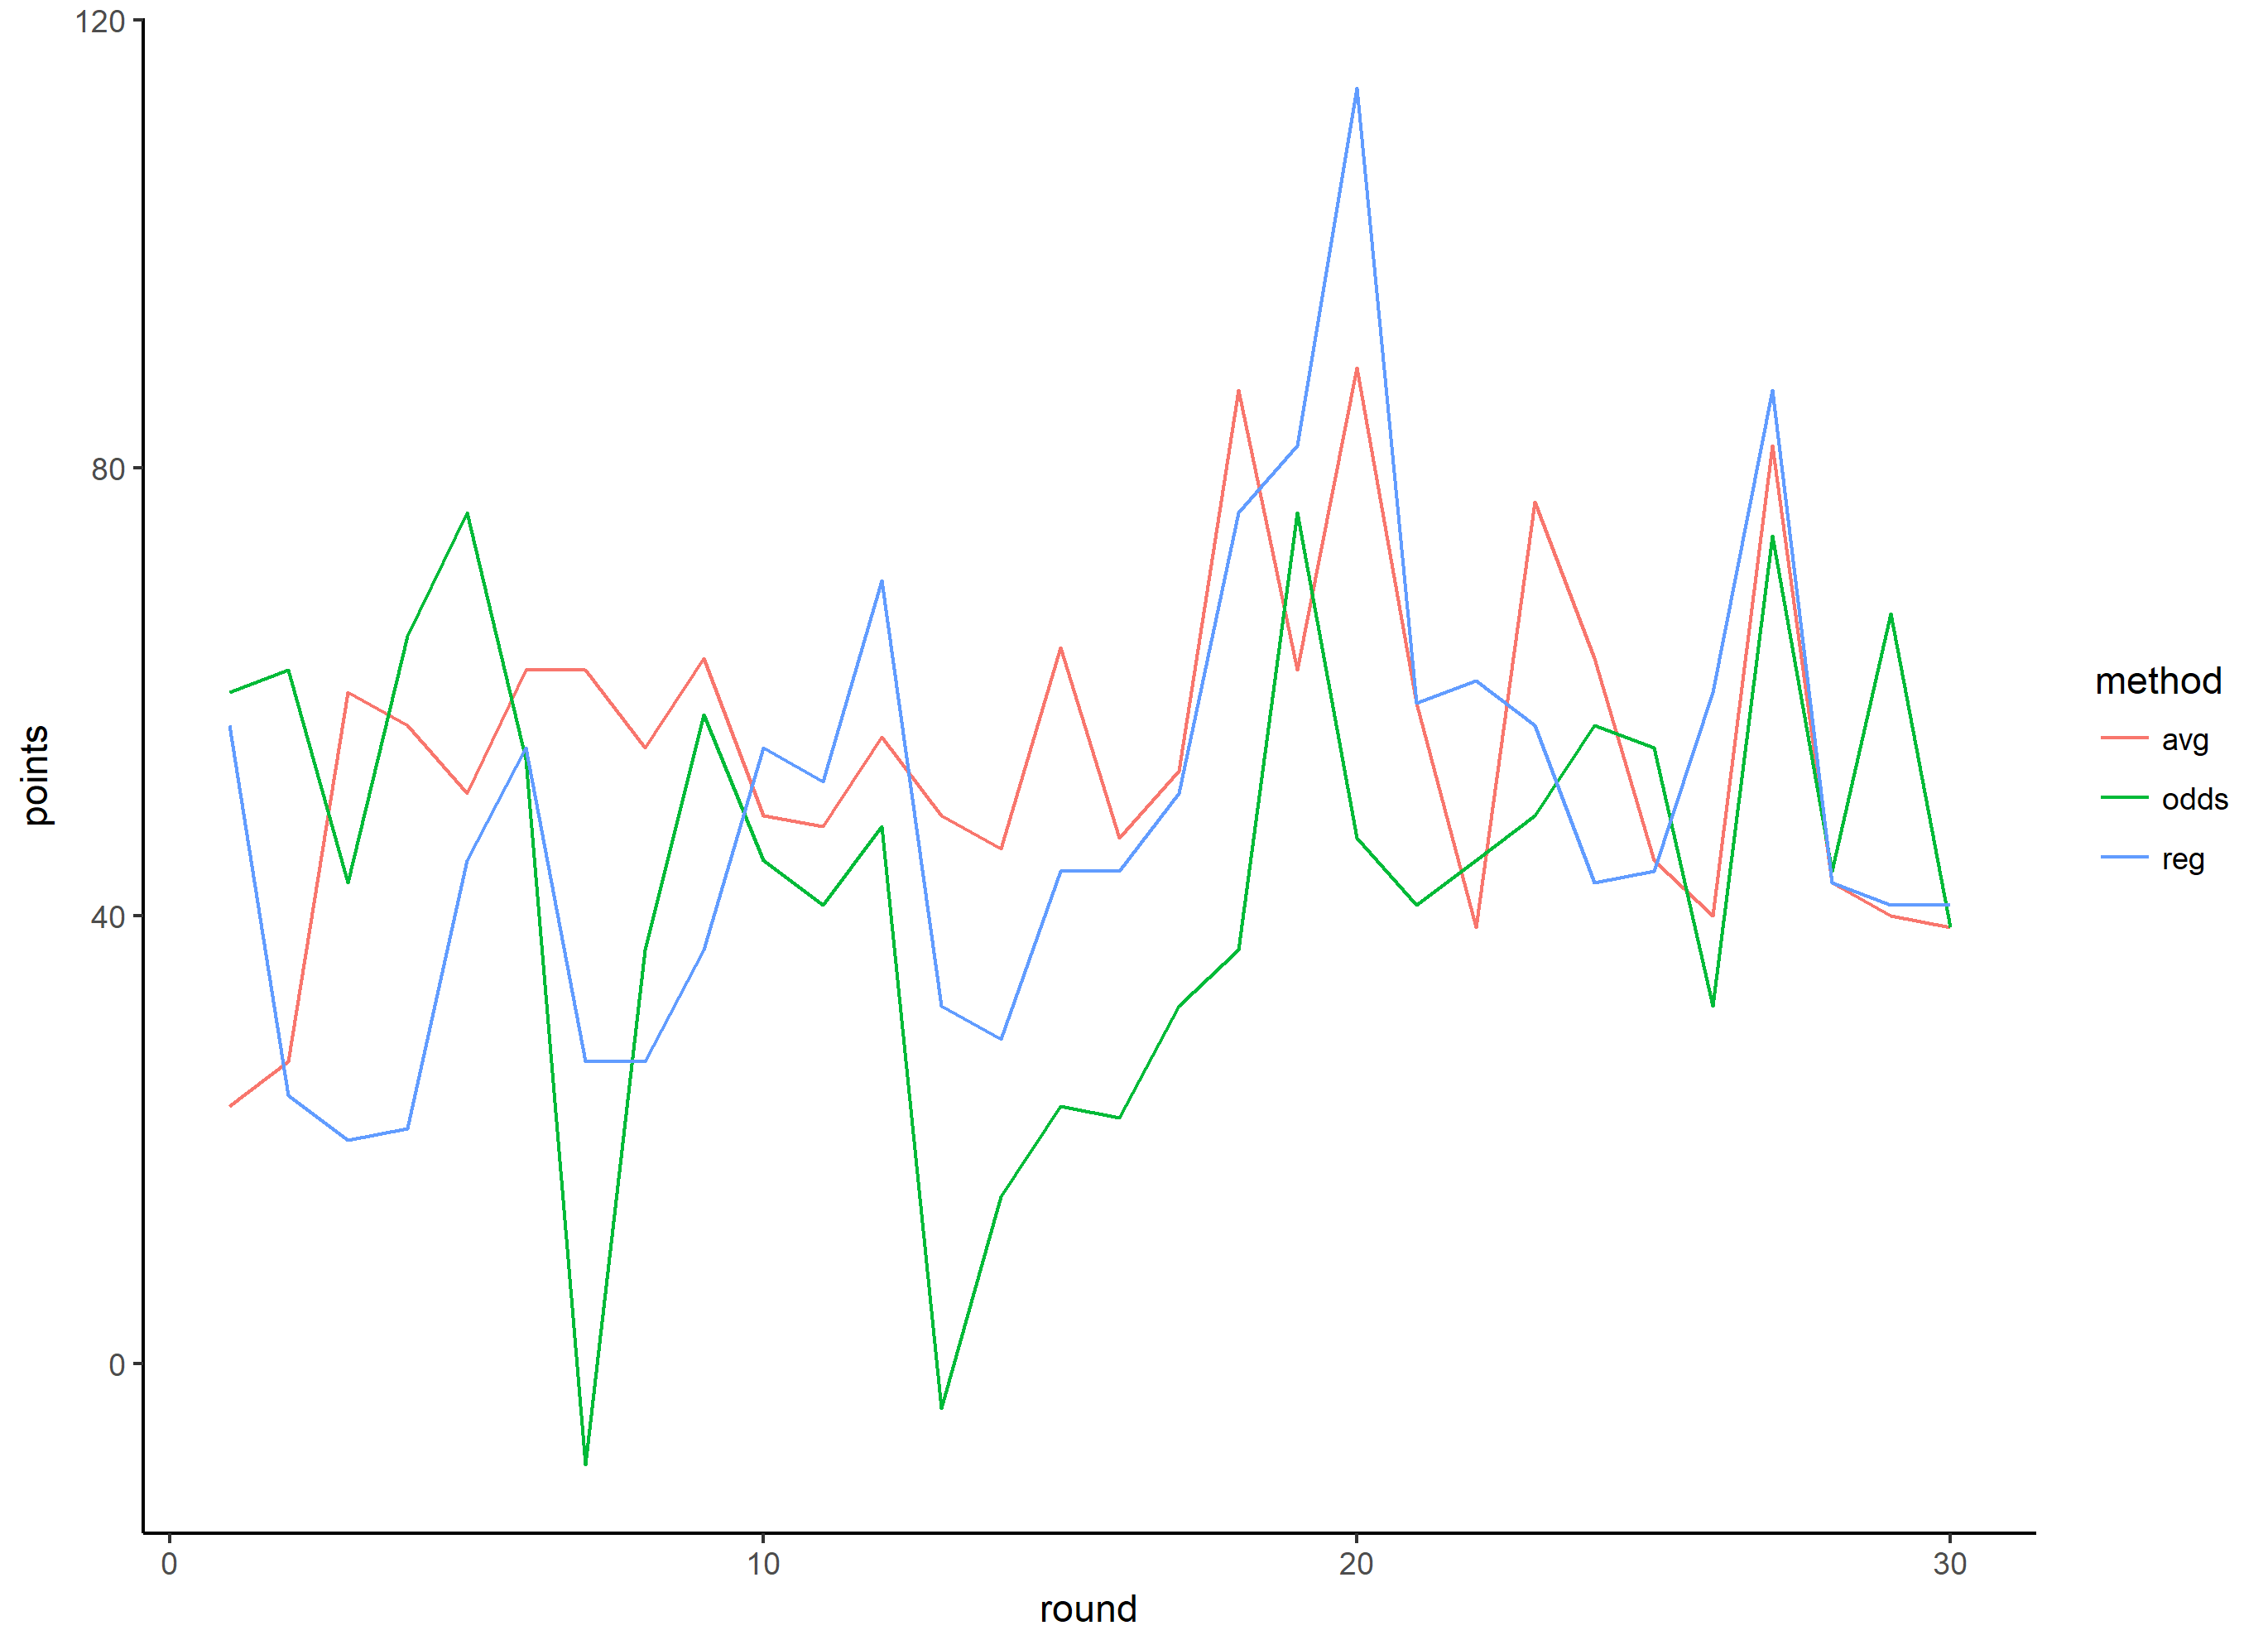
\includegraphics[scale=0.5]{fig/chapter_7/comparison_methods.png}
    \caption{Plot of the results for the different forecasting methods.}
\label{fig:res_comp_dis_gamechips}    
\end{figure}

Comparisons of the overall ranking are made in terms of mean points obtained. This is done because we have considered 31 gameweeks for the Odds method and 35 gameweeks for the two other methods. From Table \ref{tab:res_dis_gamechips}, we see that the Modified Average and the Odds method outperform the Regression method. Moreover, it is clear the mean number of penalized transfers vary considerably between the methods. The difference between the Modified Average and Regression is particularly apparent. 

\begin{table}[H]
\centering
\resizebox{\columnwidth}{!}{%
\begin{tabular}{|l|c|c|c|c|c|}
\hline
Solution method     & Total points & Mean & St.Dev  & Overall ranking & \makecell{Mean penalized \\ transfers}    \\
\hline
Modified Average    & 1916         & 54.74 & 15.85 & Top 8\%   & 0.23       \\
Regression          & 1765         & 50.43 & 20.73 & Top 30\%  & 1.80       \\
Odds (31 gameweeks) & 1650         & 53.23 & 13.94 & Top 13\%  & 0.81       \\
%Odds (28 gameweeks) & 1320         & 47.14 & & Top 47\%  & 0.39       \\
\hline
\end{tabular}%
}
\caption{Results disregarding gamechips.}
\label{tab:res_dis_gamechips}
\end{table}



\begin{comment}
However, from Figure \ref{fig:res_comp_dis_gamechips} it is evident that the Odds method performs better than the two other methods in the first 4 gameweeks. Furthermore, its performance varies significantly during the first half of the season. Note that the odds obtains negative points in gameweek 7 and 13. These were the gameweeks where odds data were missing. As for the Modified Average, its performance increases in the third gameweek. From that point on, the performance stabilizes until gameweek 17, where it increases heavily. Throughout the rest of the season, the Modified Average's performance is greatly improved, reaching scores above 80 points in diverse gameweeks. From Figure \ref{fig:res_comp_dis_gamechips} its observable that the performance of the Regression method is very weak in the first third of the season. However, it tends to increase over the length of the season.
\end{comment}
 

\subsubsection{Modified Average}
\begin{comment}
The Modified Average reaches a total score of 1916 points in the first 35 gameweeks, yielding a mean of 54.74 points per gameweek. In terms of the overall FPL ranking, the Modified Average finishes in the top 8\%.

\newpar
\end{comment}


From Figure \ref{fig:res_comp_dis_gamechips}, it is evident that the Modified Average performs poorly in the first two gameweeks. A reasonable explanation is that the forecasts are based on the previous season. Also, several players are not taken into consideration in the first gameweeks, for instance due to promotions and international transfers. In fact, the Modified Average selects Gary Cahill and Cesc Fabregas, who both received a red card, in the first gameweek. With Cahill selected as captain, they deducted a total of -7 points.

\newpar

It is observable that the weekly results tend to stabilize from gameweek 3 to gameweek 18. This can stem from the fact that forecasts now include the realized points from previous gameweeks in the 2017/2018 season. Hence, the forecasting method is able to select the players who had a good start to the season. In addition, the transferred players from outside Premier League, including players from newly promoted teams, are now assigned expected points.

\newpar

From gameweek 19 to gameweek 35, the Modified Average improves its performance compared to that in the first part of the season. Again, a plausible explanation is that the forecasts are better, by for instance being able to capture which players are performing consistently well. Moreover, the performance fluctuates more in gameweek 19 to gameweek 35. One sensible reason is the emergence of blank and double gameweeks. 


\subsubsection{Regression}

\begin{comment}
The Regression method reaches a total score of 1765 points in the first 35 gameweeks, yielding a mean of 50.43 points per gameweek. In terms of the overall FPL ranking, the Regression method finishes in the top 30\%.

\newpar
\end{comment}


The Regression method displays a higher variance than the other methods, and reaches the highest weekly realization. However, the method is outperform by the two other methods in terms of mean. The weakest weekly performances are obtained in the beginning of the season. This is perhaps explained by the fact the each player is listed with low values for variables such as goals, assists,  saves etc, making it hard to distinguish the players from each other. Also, data for the newly promoted teams are scarce, thus limiting possibilities. The method achieves its highest weekly score in gameweek 20, earning 114 points. By comparison, the best overall manager earned 156 points, but played the Triple Captain. Adjusting for the gamechip use, the best manager earned 137 points, leaving a gap of 23 points.

\subsubsection{Odds}
\begin{comment}
The Odds method reaches a total score of 1331 points for 30 gameweeks, and 1320 for 28 gameweeks, yielding a mean of 44.37 and 47.14 points per gameweek respectively. In terms of the overall FPL ranking, the Odds method finishes in the top 47\% when 28 gameweeks are considered.
\end{comment}


\newpar

The Odds method outperforms the other methods in the first gameweek and has the lowest variance. One explanation is that for the Odds method, the forecasts of points are solely based on bookmakers predictions. Since bookmakers are professional, it is not expected that their forecasts will improve greatly over the season. Of course, bookmakers will adjust their calculations based on recent performance of players and teams. However, these adjustment will not be as critical as the adjustments for the two other solution methods. 

\newpar

The Odds method is beaten by the Modified Average method. However, this does not mean that bookmakers are poor at setting odds. Remember that bookmakers are profit-seekers, and that the odds they set does not necessarily transfer into real probabilities, but are probably lower. Also, the method has a disadvantage in that the data limits us to make forecasts only for one gameweek ahead. That is, the sub-horizon must be equal one.


\subsubsection{Discussion}

The Odds method performs best over the first five gameweeks. As mentioned, the Odds method is based on bookmakers odds, and is not as heavily influenced by past season's performance as in the Modified Average and Regression method. In fact, from the previous season's Dream team, i.e. the 11 players that collected most points, only one player had a score above two points in the first gameweek. In addition, the Odds method does not exclude players due to promotion or transfers to Premier League ahead of the season. Furthermore, the Modified Average method outperforms the other methods from gameweek 5-10. One possible reason is that now, the whole track-length is founded in the 2017/2018 season.

\newpar

It appears as if the Regression method is more varying in its performance than the two other methods. This is also evident from the standard deviation presented in Table \ref{tab:res_dis_gamechips}. One explanation is that the Regression method does not account for recent performance in as a direct manner as the Modified Average method does by averaging points in the last rounds. Hence the low variability is explainable. Moreover, the Odds method has the lowest standard deviation. A possible explanation is that the odds are set by the standard procedures of professional bookmakers, while the other methods are solely based on data and will to a larger degree incorporate extreme and unexpected previous events.

\newpar

As evident from Table \ref{tab:res_dis_gamechips}, the number penalized transfers is quite different between the methods. In particular, it is high for the Regression method. In fact, it can be argued that the higher penalty term incorporated for Modified Average is only a compensation for inaccurate forecasts. Thus, it appears as if the Regression method in particular could also benefit from a parameter-tuning approach with respect to penalized transfers. However, this was constrained by the lack of data. Hence, it is arguable that it is unfair to compare the performance of the Regression method with the Modified Average method.

\newpar

Without the gamechips, it appears as if it is achievable to reach to 10\%-15\% in terms of overall ranking with our forecasting-based optimization model for the FPL.




\begin{comment}
Additionally, football is a sport with high uncertainty. Player performances are hard to predict, as factors such as opponents, home field advantage and after all luck affects the performances. 
\end{comment}


\subsubsection{Comparing Modified Average with the solution suggested by \cite{Bonomo}}




We remind reader that the Modified Average method is inspired by the solution approach suggested for the Argentinian Fantasy Football by \cite{Bonomo}. Therefore, we find it interesting to compare the performance of the two different methods. From Figure \ref{fig:avg_vs_bon} and Table \ref{tab:bonomo_mofidified_average}, it is clear that the Modified Average outperforms the approach suggested by \cite{Bonomo}.\cite{Bonomo} set the track-length to 3 and the sub-horizon to 1. Note, however, that the Argentinian fantasy league does not penalize transfers. Therefore, the penalty term is set to 4 as this is stated by the game rules of FPL. Thus, the basis for comparison is somewhat compromised and one should be careful not to draw too categorical statements about the two methods. Regardless, it is apparent that for the 2017/2018, the Modified Average performs constantly better and is a potential improvement of the method.

\begin{figure}[H]
    \centering
    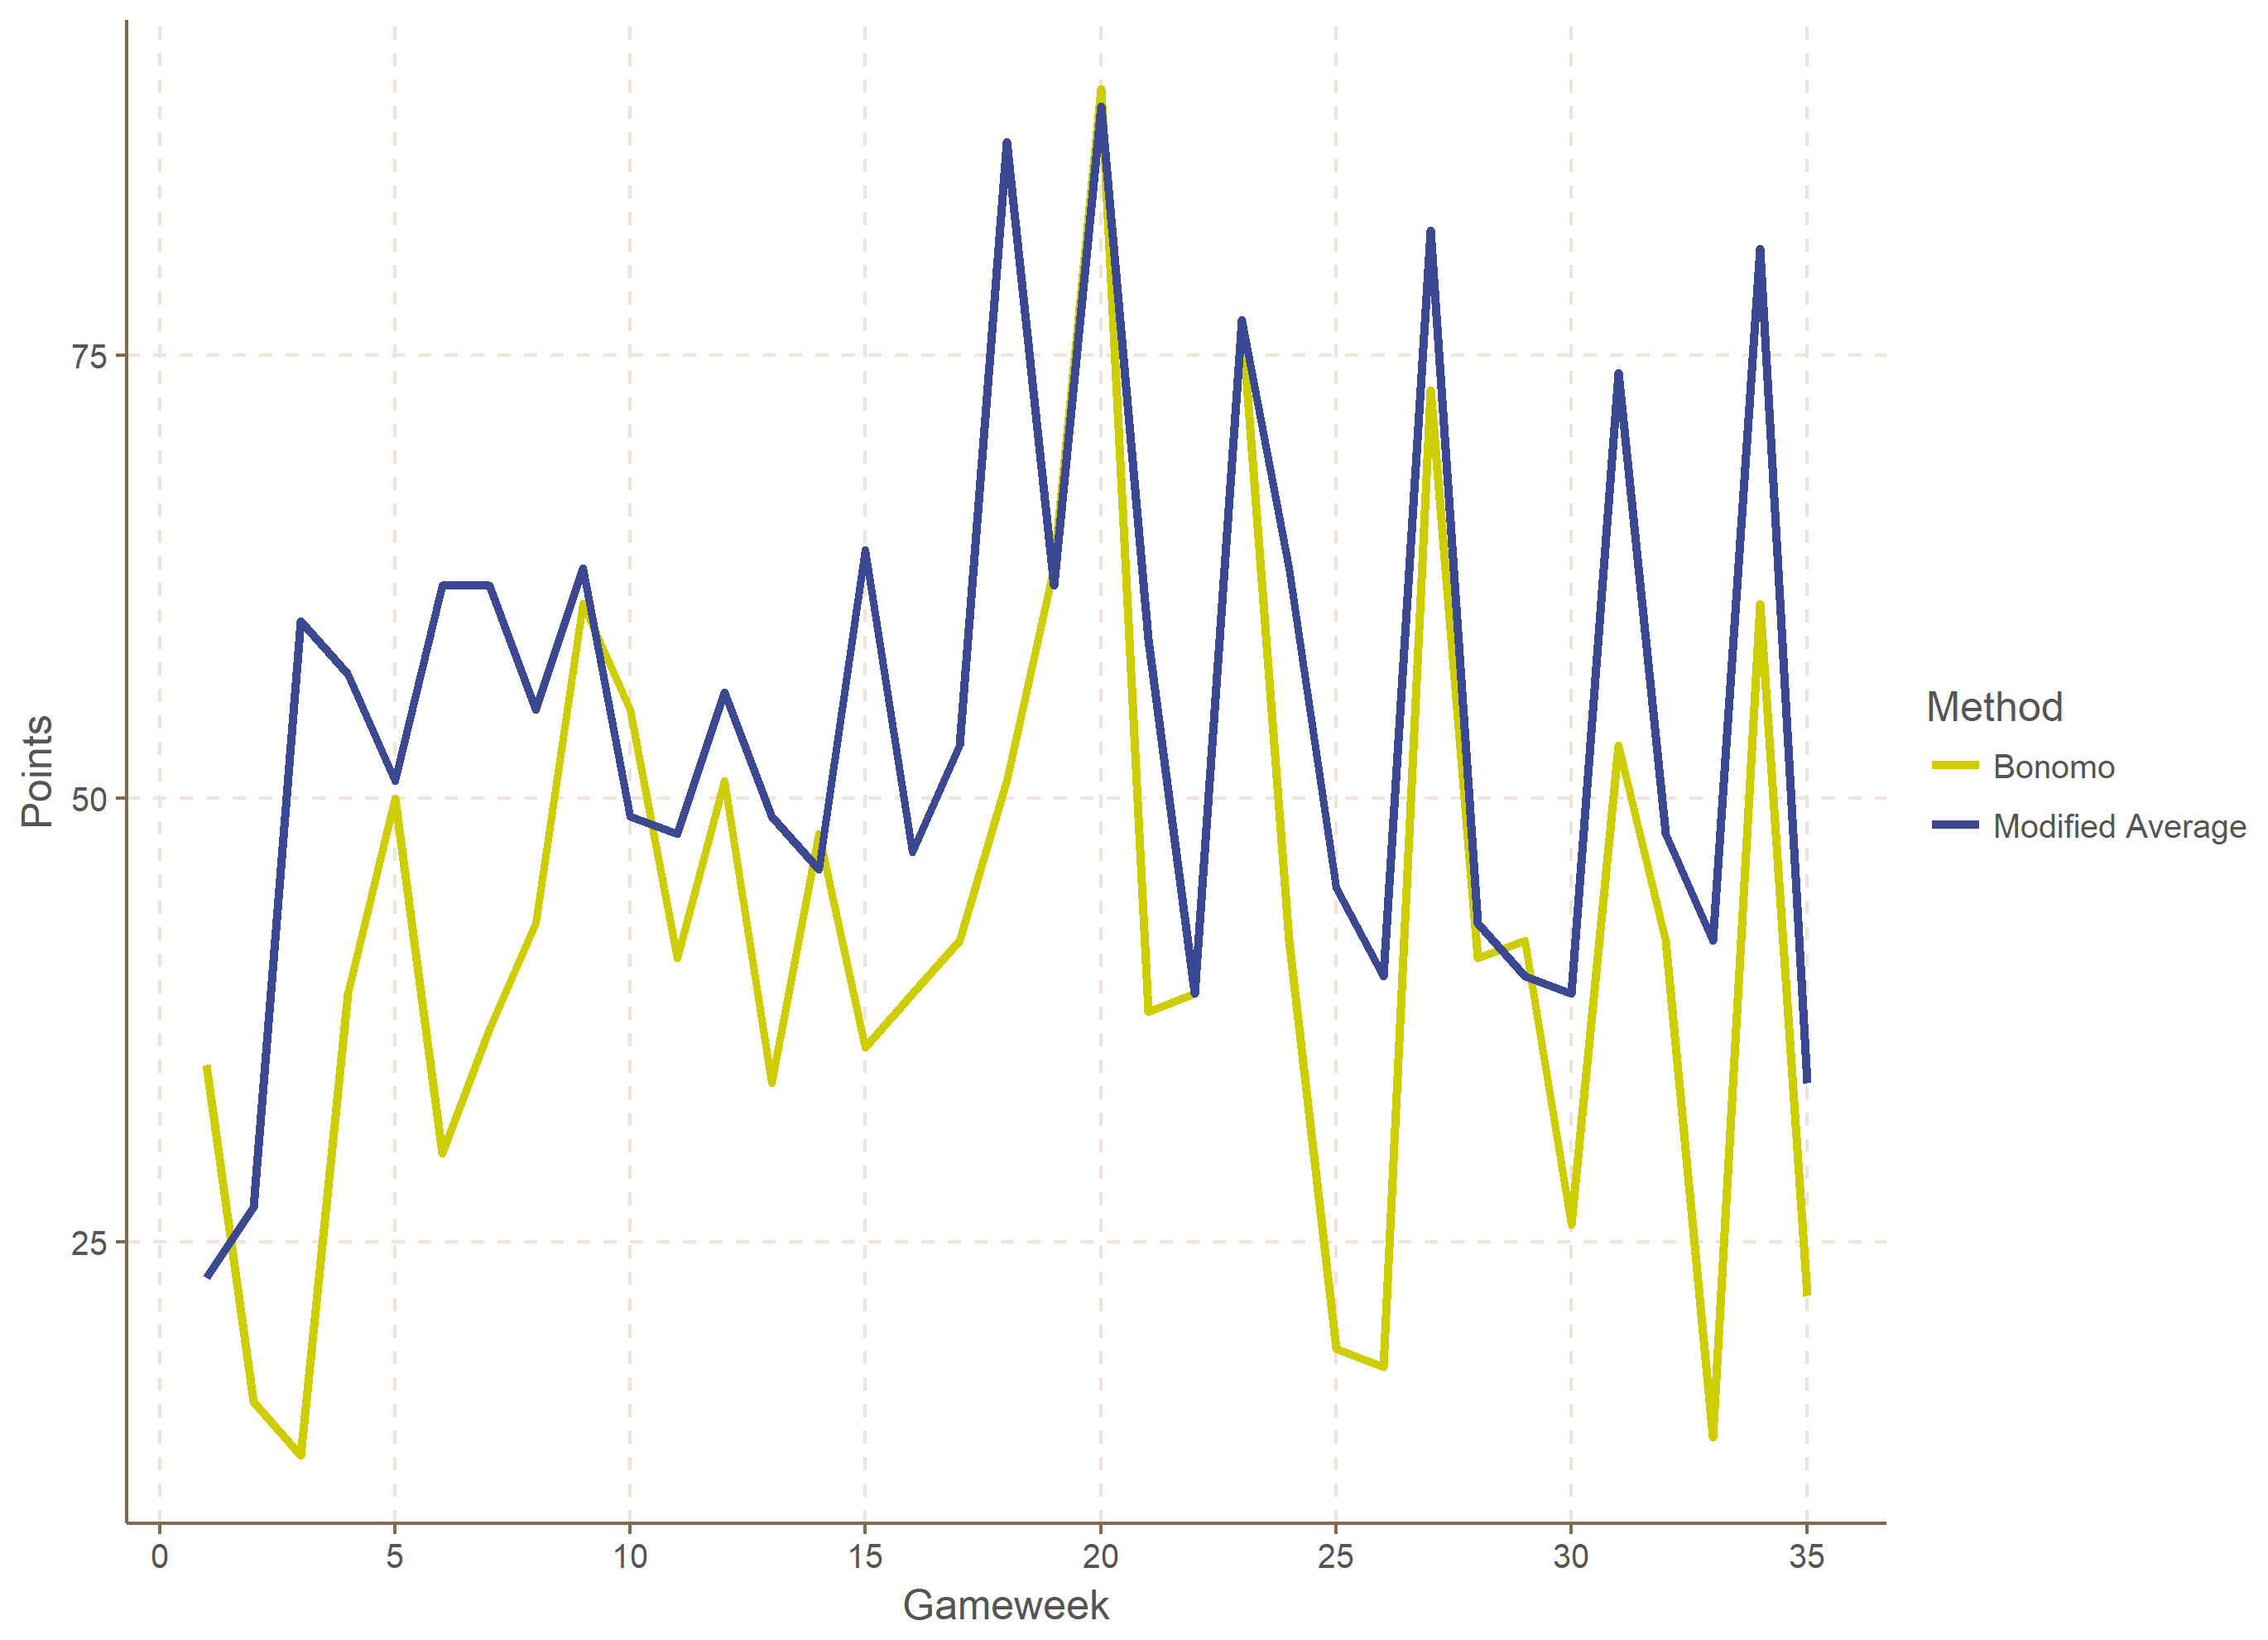
\includegraphics[scale=0.5]{fig/chapter_7/bon_gc_no_gc.png}
    \caption{Comparing performance of Modified Average with the solution approach suggested by \cite{Bonomo}.}
\label{fig:avg_vs_bon}    
\end{figure}

\begin{table}[H]
\centering
\resizebox{\columnwidth}{!}{%
\begin{tabular}{|l|c|c|c|c|c|}
\hline
Solution method     & Total points & Mean & St.Dev  & Overall ranking & \makecell{Mean penalized \\ transfers}     \\
\hline
Modified Average    & 1916         & 54.74 & 15.85 & Top 8\%   & 0.23       \\
\cite{Bonomo}       & 1481         & 42.31 & 17.43 & Top 69\%  & 2.23       \\

\hline
\end{tabular}%
}
\caption{Performance of Modified Average and \cite{Bonomo}}
\label{tab:bonomo_mofidified_average}
\end{table}


\subsection{Results Including Gamechips}

In Table \ref{fig:res_comp_gamechips}, a summary of the performance of each model when including gamechips is presented. Furthermore, summarizing statistics for the Weekly Average and Top Manager is included for comparison. By comparing the mean obtained with and without gamechips, it is apparent that the effect of gamechips is not consistent for the methods.


\begin{figure}[H]
    \centering
    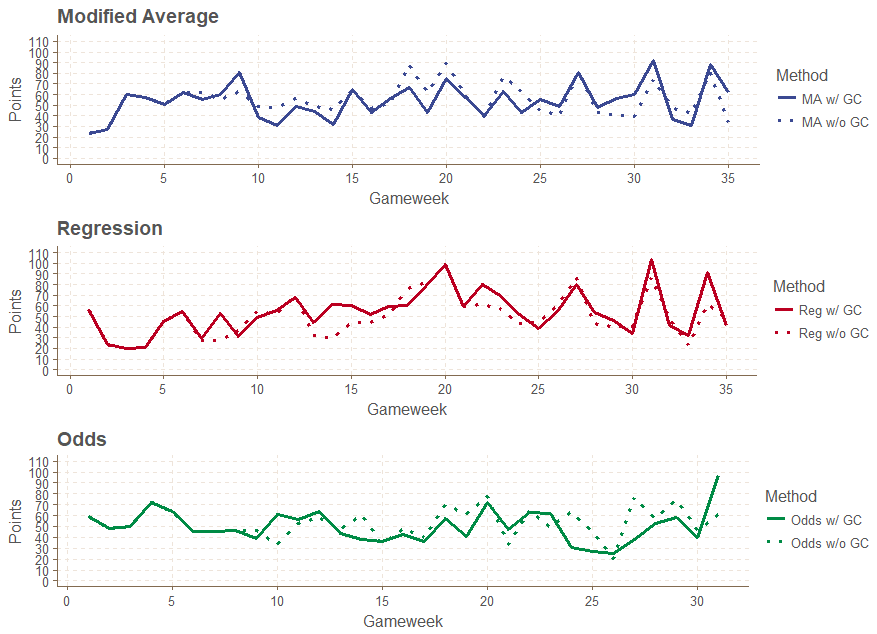
\includegraphics[scale=0.5]{fig/chapter_7/w_wo_gc_all.png}
    \caption{Comparing performance with gamechips.}
\label{fig:res_comp_gamechips}    
\end{figure}

In Figure \ref{fig:res_comp_gamechips}, each method is plotted with and without gamechips. In the following, we discuss how each gamechip have effected the solutions. Note that for each method, points obtained are similar for the first 6 gameweeks. As mentioned in Section \ref{exp_setup_gamechips} the model was allowed to use a Wildcard in gameweek 9, hence this decision was first considered in gameweek 7 due to the sub-horizon of three gameweeks. Therefore, the models make different decisions from that point on.

\begin{comment}
\begin{figure}[H]
    \centering
    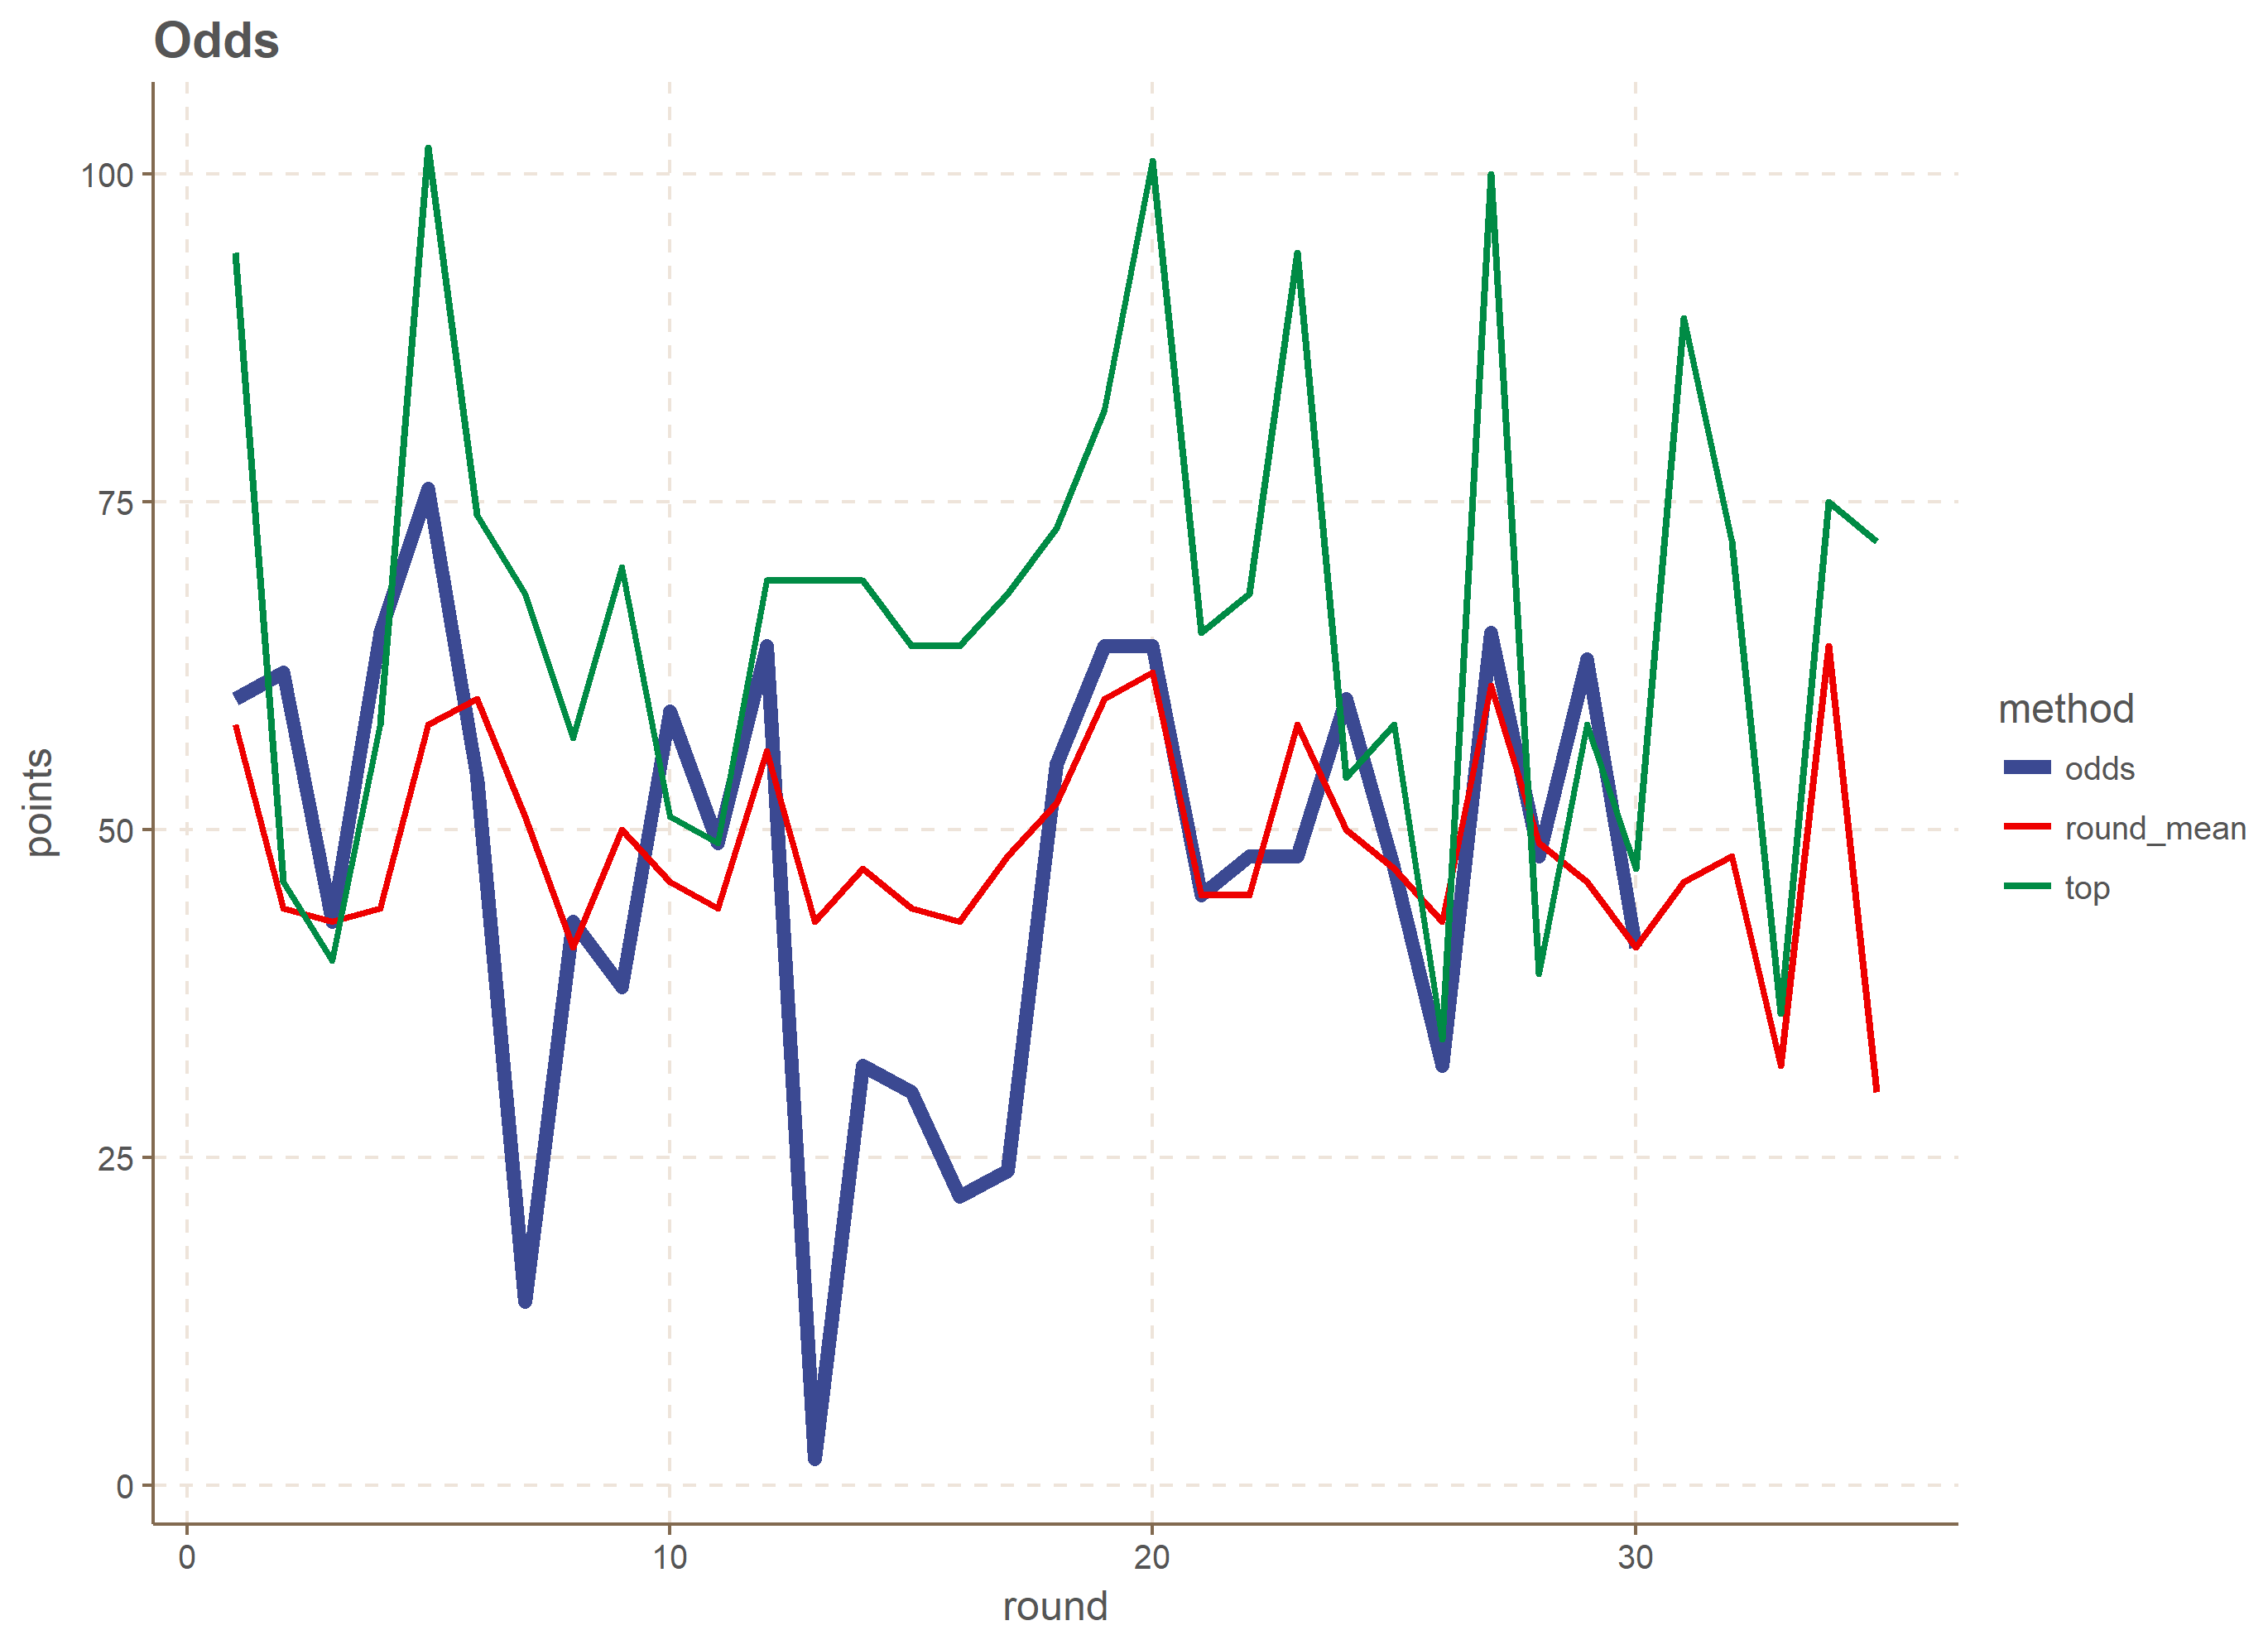
\includegraphics[scale=0.5]{fig/chapter_7/top_mean.png}
    \caption{Comparing performance with gamechips with weekly average and top manager.}
\label{fig:top_mean}    
\end{figure}
\end{comment}


\begin{table}[H]
\centering
\resizebox{\columnwidth}{!}{%
\begin{tabular}{|l|c|c|c|c|c|}
\hline
Solution method     & Total points & Mean & Std.Dev  & Overall ranking & \makecell{Mean penalized \\ transfers} \\
\hline
Modified Average    & 1881         & 53.74 & 16.62 & Top 12\%   &  0.23   \\
Regression          & 1901         & 54.31 & 20.32 & Top 10\%   &  1.20   \\
Odds (31 gameweeks) & 1557         & 50.23 & 15.17 & Top 30\%   & 0.48   \\
%Odds (28 gameweeks) & 1401         & 50.04 & 13.66 & Top 31\%   &  0.29   \\
Weekly Average      & 1699         & 48.53 & - & Top 40\%   &  - \\
Top Manager         & 2329      & 66.54 & 18.02 &  Top 1 ‰   & 0.11\\
\hline
\end{tabular}%
}
\caption{Results including gamechips.}
\label{tab:res_incl_gamechips}
\end{table}


To discuss the effect of the first Wildcard, the performance in gameweek 7 to 28 are interesting. 

To discuss the impact of the first Wildcard,  we compare performance from gameweek 7, as this is the first gameweek were decisions regarding the Wildcard are introduced. Moreover, we only measure the effect until gameweek 28, as decisions regarding the Free Hit are first introduced in gameweek 29. As seen in Table, all methods performs 

\textit{Tabell med antall bytter og prestasjon med og uten WC gw7-28}


For the Modified Average, 11 transfers were made using a Wildcard, the two teams' starting line-ups became significantly different from this point on. Unfortunately, the Wildcard had a poor impact for the upcoming gameweeks, being outperformed by the other model in 10 of the following 13 gameweeks. Further, in gameweek 22, the Triple Captain chip was used, selecting Harry Kane as the captain. However, since Kane performed poor in both matches of the double gameweek, the Triple Captain had a rather weak impact on the total points gained. From this point on, the model including the gamechips tends to outperform the other for the rest of the season. In gameweek 31, it plays the Free Hit due to a blank gameweek. For this particular gameweek, it greatly outperforms the other model as the Free Hit ensured that each player on the team was featured in that gameweek. In comparison, the model without the gamechips only had 5 players that were featured in gameweek 31. The second Wildcard was played in gameweek 33, preparing for the double gameweek 34 and the blank gameweek 35. From figure \ref{fig:avg_gc_no_gc} its observable that usage of the Bench Boost yielded a total of 88 points in gameweek 34. Thus, it outperformed the model disregarding  gamechips with 7 points in gameweek 34. 

\textit{Tabell med antall bytter og prestasjon med og uten TC gw 20-22}

\newpar

\textit{Tabell med antall bytter og prestasjon med og uten FH gw 29-31}
  
\newpar

\textit{Tabell med antall bytter og prestasjon med og uten W, BB gw 32-34} 

\newpar




\subsubsection{Discussion - effect of gamechips}



In general, the methods with gamechips does not outperform the methods without. When considering the performance of each model in gameweek 1-21, it is hard to spot the difference. 


However, the models appear to perform better in the particular gameweeks where Triple Captain, Bench Boost and Free Hit are played. This is as expected, as these gamechips are used in order to boost the performance for one gameweek. However, as we only have odds for the first 31 gameweeks, the second Wildcard and Bench Boost are not considered for the Odds method. 

\newpar

When regarding the Wildcards, it is noticeable from Figure \ref{fig:avg_gc_no_gc} that the first Wildcard have a negative impact on the Modified Average method. In fact, from gameweek 7 to gameweek 28 the model disregarding gamechips outperforms the one including them with 100 points. 
\newpar

When considering overall rank, it is worth noting that we have used all gamechips for the Modified Average and Regression, while this is not necessarily the case for other managers. 

\begin{comment}
By performing 11 transfers, the new team differs significantly from that without gamechips. The poor performance in the following gameweeks are due to weak foorcasts of future performance. Hence, the effects of the Wildcard propagates throughout the season. 
\end{comment} 

\newpar
In the Regression method, the inclusion of the first Wildcard has a slightly negative impact on the overall result. From gameweek 7 to gameweek 28, the model disregarding gamechips outperforms the one including them with 7 points. 

\newpar

As for the Odds method however, the inclusion of the first Wildcard significantly improve the performance. This is shown in Figure \ref{fig:odds_gc_no_gc}. Clearly, by comparison of Table \ref{fig:res_comp_dis_gamechips} and \ref{fig:res_comp_gamechips}, we see that the first Wildcard has a great positive effect for the Odds method. This can be stated as only the first Wildcard and the Triple Captain (which increased the captain's score by 5 points) were played in the Odds method. 

\newpar

- godt poeng: man ser i regresjonen at det er ikke tidseffekt av poeng, og det kan forklare hvorfor modified average kan gjøre dårlig siden man vil ha et stabilt lagt over en sesong. Og da, kan det også forklare hvorfor wildcard gjør det bedre på regresjonen. 

- godt poeng: når human fpl managers bruker wildcard vil man ikke ha inn formspillere, som hegazi, og man vil til en større grad bygge et lag for mange uker fremover. med en subhorizon på 3 uker, er ikke dette helt gunstig. 

- godt poeng: at man fikser modellen til å bruke gamechippene i visse uker og dermed minsker løsningsrommet og dermed er det ikke rart at man får sub-optimale løsninger. 

Finally, from Figure \ref{fig:avg_gc_no_gc} and \ref{fig:reg_gc_no_gc} it is evident that the combination of the second Wildcard and the Bench Boost had a positive impact on both the Modified Average and the Regression method. This may provide evidence that combining the Second Wildcard and Bench Boost yields a positive result. Moreover, it is noticable that the second Wildcard had a great positive impact for the blank gameweek 35 in both methods. 

\subsection{Summary}
Here we present a table that summarizes the results from the three different approaches. 

\newpar

As evident from Table \ref{tab:res_dis_gamechips} and \ref{tab:res_incl_gamechips}, the solution method disregarding gamechips outperforms that of including gamechips, obtaining mean scores of 54.74 and 53.74 respectively. Furthermore, in terms of the overall Fantasy Premier League rankings, they would finish among the top 8\% and 12\% respectively. 

\newpar

Figure \ref{fig:reg_gc_no_gc} provides a comparison of the results from the Regression method when gamechips are included and disregarded. As evident from Table \ref{tab:res_dis_gamechips} and \ref{tab:res_incl_gamechips}, the solution method including gamechips outperforms that of disregarding them, obtaining mean scores of 53.97 and 50.43 respectively. Furthermore, in terms of the overall Fantasy Premier League rankings, they would finish among the top 11\% and 30\% respectively. 

\newpar

As evident from Table \ref{tab:res_dis_gamechips} and \ref{tab:res_incl_gamechips}, the solution method including gamechips outperforms that of disregarding gamechips, obtaining mean scores of 50.24 and 47.14 respectively. Furthermore, in terms of the overall Fantasy Premier League rankings, they would finish among the top 31\% and 47\% respectively. 

\newpar

In general, a solution method using odds is expected to perform evenly throughout the season, due to the consistency of predictions. Compared to the Modified Average and the Regression methods, this is evident as the Odds method has lower vertices. Moreover, as shown in Table \ref{tab:res_incl_gamechips}, the Odds method has lower variance in terms of mean performance when disregarding gameweek 7 and gameweek 13.  

\newpar

Again, we stress the fact that no general conclusion can be made as this is tested on data only for one season. However, the performance show that there are potential in both the problem and the solution method.  

\begin{comment}
\section{Recommendations for human FPL managers}
- hvilke anbefalinger kan man gi til fpl managere? 
     * hvilke formasjon går igjen i løsningene. lønner det seg med forsvarsspillere eller angrepsspillere?  
    * er budsjettet alltid oppfylt? og hvordan utvikler verdien til laget seg over sesongen? 
    
    - Tabell over Formasjon i optimal solution. 



\begin{table}[H]
\centering
\caption{Results of total sum, average, total sum best player. Model without variance.}
\begin{tabular}{llllllll}
& Average Argentina & Average Improved & Odds & Regression  & Average Players & Best Player & Exact\\
Total sum  & NA  & NA & NA & NA & NA & NA & NA \\
\end{tabular}
\end{table}
\end{comment}

\begin{comment}
Good discussion points: 
\begin{enumerate}
    \item hvis man legger restriksjon på formasjon. Hvilke formasjon gir mest poeng?
    \item når bruker man de forskjellige chippene, og hvor effektive er de?  
\end{enumerate}
\end{comment}


\section{Risk Handling}

In this section the element of risk handling is added to the mathematical model to analyze its effect. The constraints \ref{eq:variance} to \ref{eq:variance_p_p_dash_beta} are included in the mathematical model formulated in Section \ref{mathematical_model} and run with changing $\sigma_{0}^2 \in [\underline{\sigma}, \overline{\sigma}]$. The objective of adding the constraints is the add on of \textit{diversification}, a risk management technique which as the purpose of on average yielding higher returns(expected points) and give a lower risk.

\newpar

The method with the best results from previous sections is used as forecasting method. Hence, Modified average is used. The aim is to discuss its effect on the solution, and examine the performance to see if there are any similarities with the variance effect in portfolio optimization. It is important to emphasize that one can not take any general conclusions on the impact, as this is bases on realization of points in one season. Nevertheless, a season includes 35 data points on 625 players, and consequently useful insight is obtainable from such analysis.  

\newpar

There are two interesting dependencies to analyze: the effect the variation of threshold has on expected points, and the effect the variation of threshold has on realized points.

\newpar

The computational time is increased considerably when including constraints \ref{eq:variance} to \ref{eq:variance_p_p_dash_beta}. This is explainable since these are quite heavy constraints. The computational time varies from 26 min to 17 min for the threshold $\underline{\sigma}$ to $\overline{\sigma}$, respectively. 

\newpar

The mathematical model maximizes based on player's expected points, and the variance is estimated by the use of historical data. Hence, one would assume that when the threshold is decreased, the expected value of the team also decreases. This would coincide to the efficient frontier in portfolio optimization, where one obtains the optimal set of portfolios which gives the highest expected points for a certain level of risk, i.e. variance. In Figure \ref{fig:threshold_obj_value}, the expected points are plotted against threshold. From the figure one can see that it violates the prediction of a perfect curve, as there are some outliers. One explanation could be the handling of input for players which have not featured in the FPL before. This were handled by setting their variance to the average. In the first rounds, there is a big chance that there are players with the same expected points, and same empirical variance since we set the variance to average for the players we do not have data on. Hence, the model has several solutions with the same expected value and consequently when we set a unlimited threshold the results differs with the results without the threshold. This is a drawback with how we handle forecast and estimation on players we do not have data on, and an alternative approach which takes this issue into account wold be interesting. 

\newpar

An interesting question is how much is the impact the restriction on variance has on the expected value. It is reasonable to say that a steeper curve suggests a bigger impact, and the less steeper curve suggest a smaller impact. Figure \ref{fig:threshold_obj_value_linear_curve} suggests that the impact is not that severe. This moves to the discussion of how important it is actually to include variance in FPL decisions. This is difficult to say before we have examined the impact on the realized points, which will be further discussed. 

\newpar

The case with realized points is slightly different from expected value. One would expect a similar impact of the variance constraints, however there is naturally a bigger possibility of outliers. Figure \ref{fig:threshold_mean} shows that there is a negative trend when the thresholds is decreased. This coincides well with the logic of portfolio optimization. In addition, there is also one case of actually obtaining better results. Threshold of 5000 gives a mean of 54.7 which is better than without the variance constraints. 

\newpar

In the end, it is interesting to investigate how different the teams actually are with the introduction of variance constraints. Do the model choose players which are stable and always achieves a certain amount of points? And, do the model choose players which plays for opposing teams? Or the model always try to pick players which do not play against each other? In general, do the behaviour of the model imitate the analogy of diversification in portfolio management? If so, this is a great finding. 


\begin{figure}[H]
    \centering
    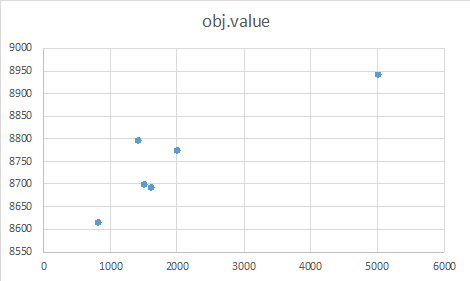
\includegraphics[scale=0.75]{fig/chapter_7/threshold_obj_value.png}
    \caption{Threshold plotted against objective value in the mathematical model.}
\label{fig:threshold_obj_value}    
\end{figure}

\begin{figure}[H]
    \centering
    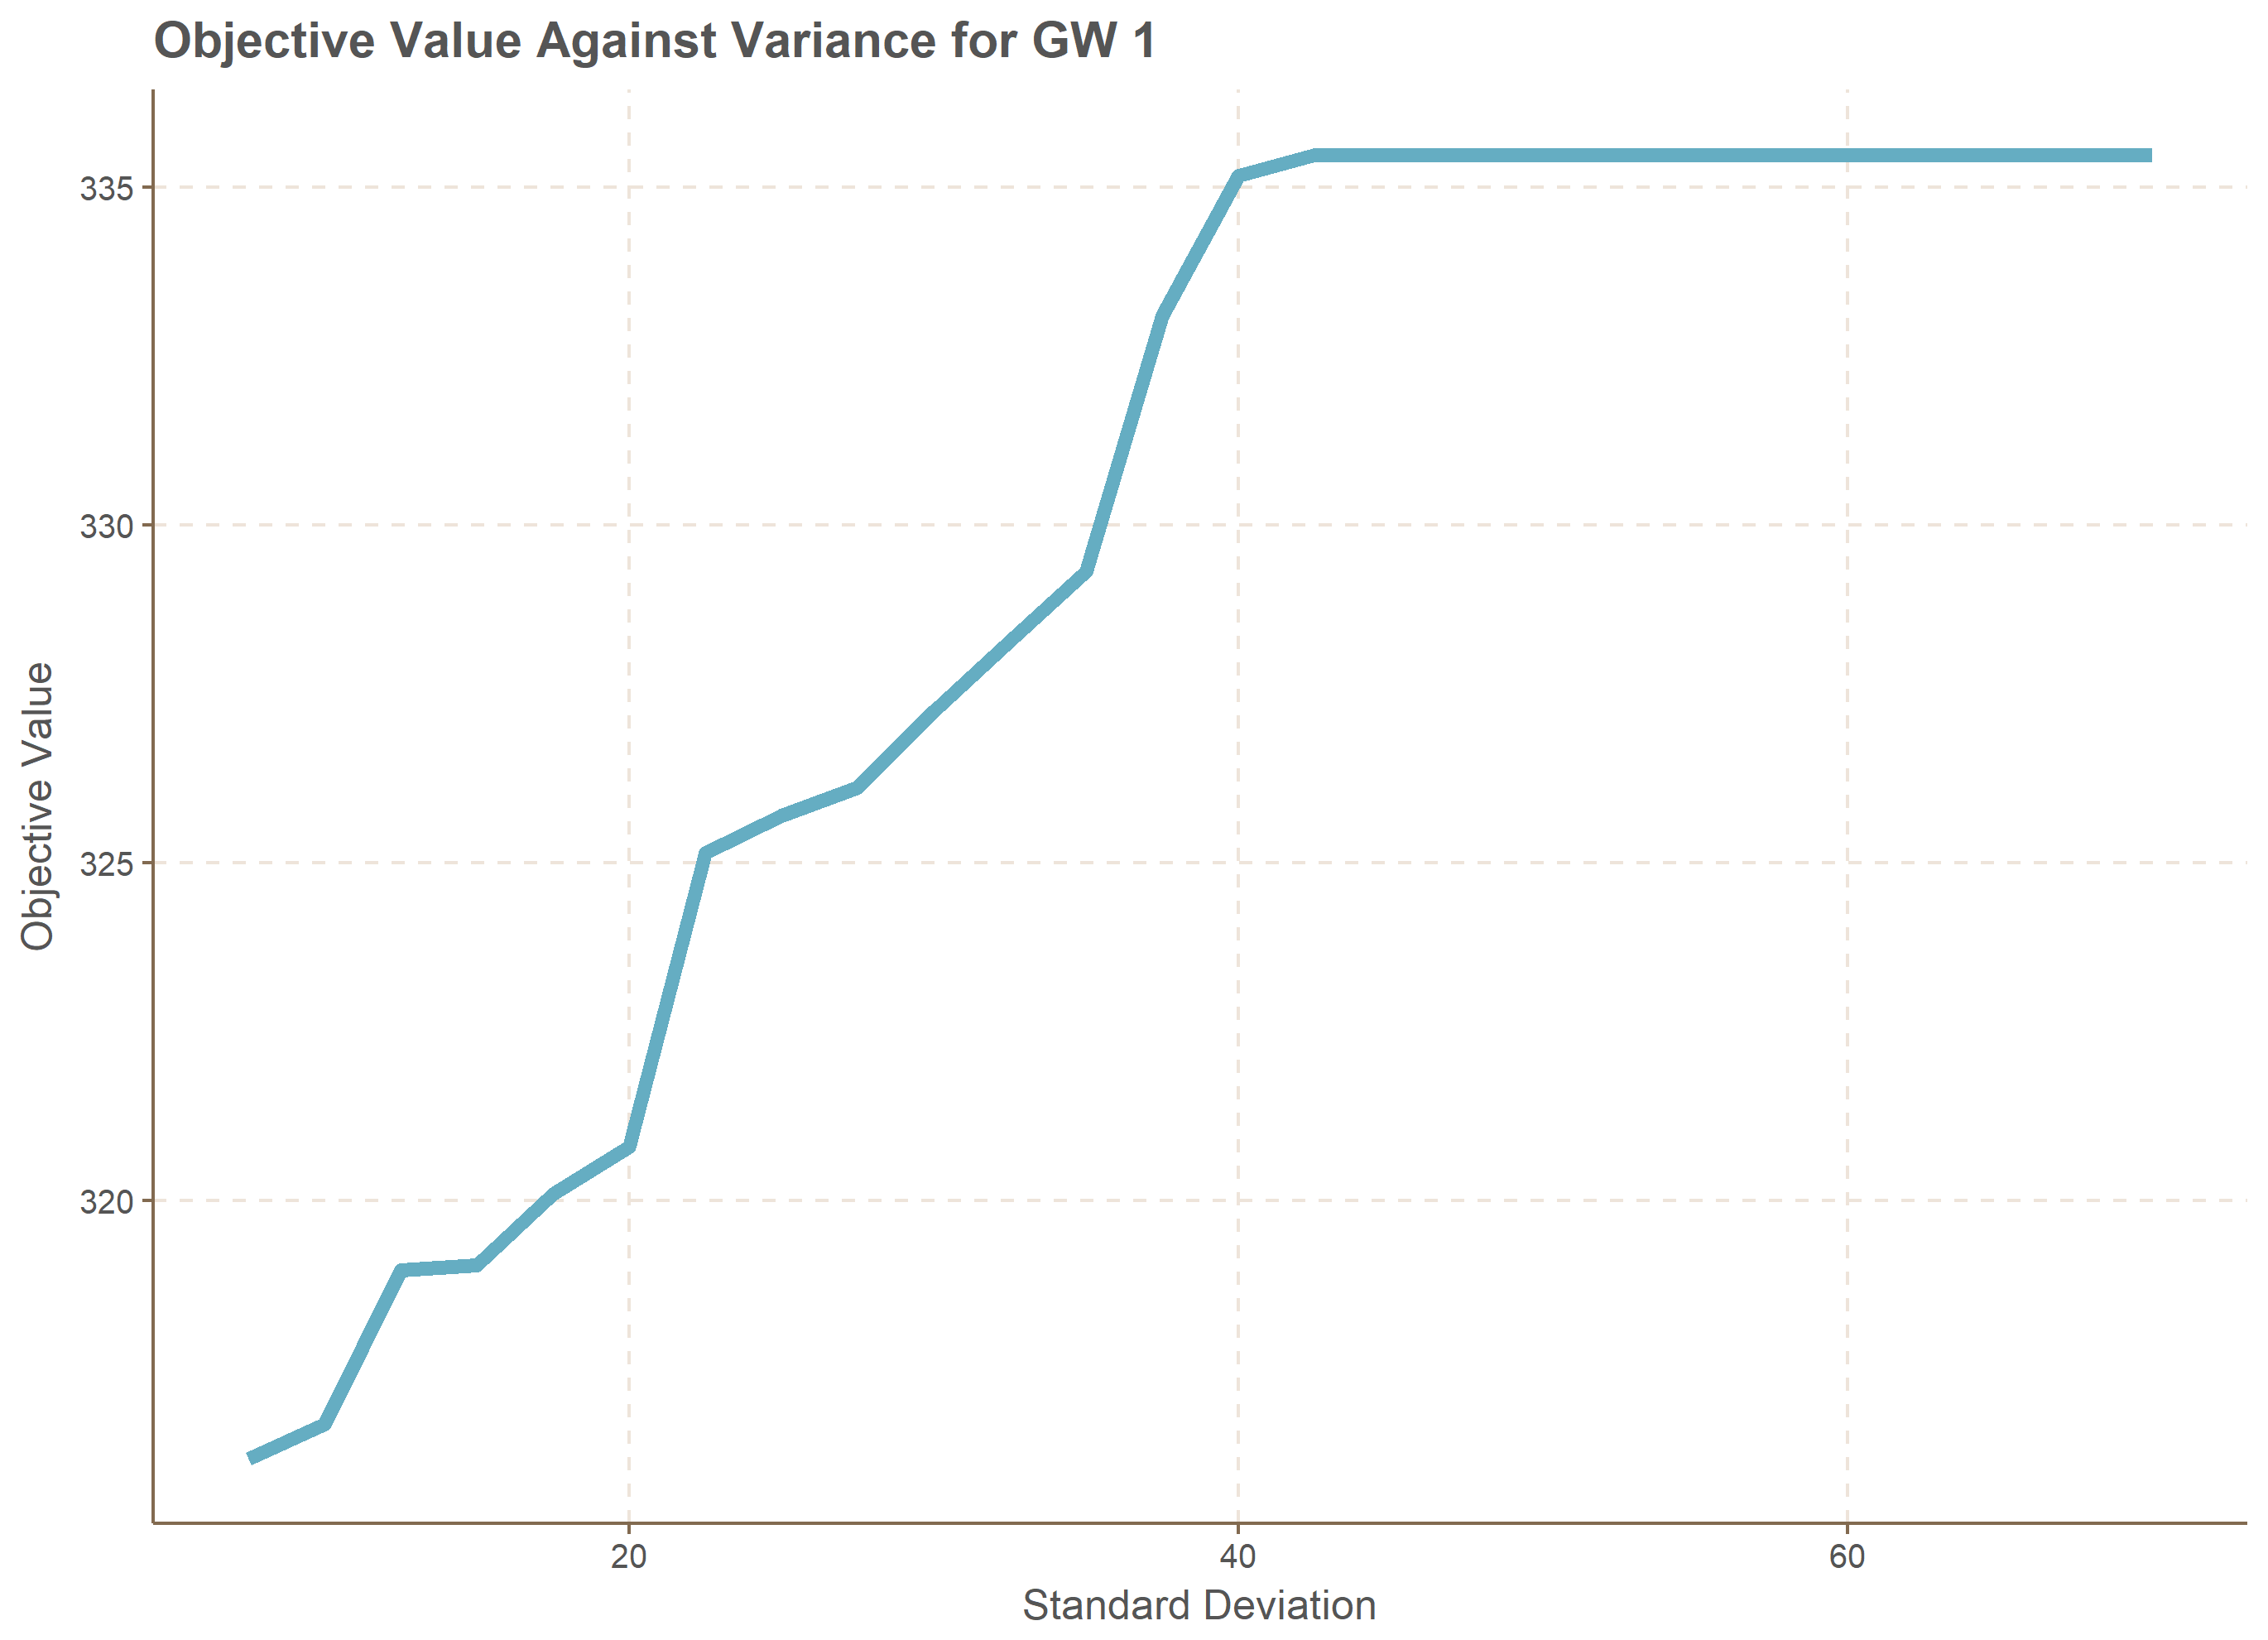
\includegraphics[scale=0.75]{fig/chapter_7/GW1_var.png}
    \caption{Linear curve of the data points in Figure \ref{fig:threshold_obj_value}.}
\label{fig:threshold_obj_value_linear_curve}    
\end{figure}


\begin{figure}[H]
    \centering
    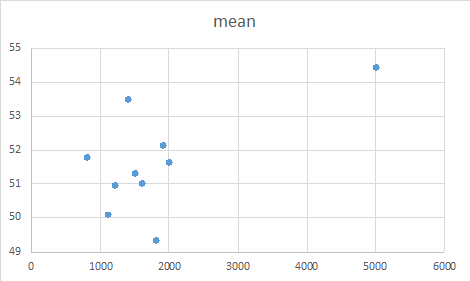
\includegraphics[scale=0.75]{fig/chapter_7/threshold_mean.png}
    \caption{Threshold plotted against realized points shown by mean.}
\label{fig:threshold_mean}    
\end{figure}

\begin{comment}
\begin{enumerate}
    \item plot with the objective value and threshold. the objective value is the accumulated objective value of the model run over all gameweeks. 
    \item explanation of the graph and discussion 
    \item plot with the realized points and threshold. 
    \item explanation of the graph and discussion. 
    \item 
\end{enumerate}
\end{comment}





\begin{comment}

\begin{table}[H]
\centering
\begin{tabular}{@{}lll@{}}
\toprule
$\sigma^2$ & Expected Points GW1 & Computational Time (seconds) \\ \midrule
$5^2$       & 314.185              & 315.917            \\
$7.5^2$     & 317.951             & 207.44             \\
$10^2$      & 318.84              & 919.085            \\
$12.5^2$    & 318.759             & 140.888            \\
$15^2$      & 319.619             & 1005.57            \\
$17.5^2$    & 322.155             & 183.62             \\
$20^2$       & 323.391             & 848.809            \\
$22.5^2$ & 324.712             & 103.374            \\
$25^2$       & 327.164             & 685.687            \\
$27.5^2$& 325.11              & 140.167            \\
$30^2$       & 327.445             & 590.303            \\
$32.5^2$     & 330.43              & 116.318            \\
$35^2$      & 329.316             & 629.958            \\
$37.5^2$     & 333.1               & 82.781             \\
$40^2$      & 335.164             & 105.532            \\
$42.5^2$    & 335.475             & 27.688             \\
$45^2$      & 335.475             & 102.61             \\
$47.5^2$    & 335.475             & 27.403             \\
$50^2$      & 335.475             & 103.023            \\
$52.5^2$    & 335.475             & 27.621             \\
$55^2$      & 335.475             & 94.686             \\
$57.5^2$     & 335.475             & 27.382             \\
$60^2$      & 335.475             & 86.712             \\
$62.5^2$     & 335.475             & 27.5               \\
$65^2$      & 335.475             & 65.378             \\
$67.5^2$    & 335.475             & 21.747             \\
$70^2$      & 335.475             & 102.856            \\
$72.5^2$     & 335.475             & 27.775             \\
$75^2$      & 335.475             & 169.981            \\
$77.5^2$    & 335.475             & 27.752             \\
$80^2$      & 335.475             & 118.392            \\
$82.5^2$    & 335.475             & 27.619             \\
$85^2$      & 335.475             & 111.9              \\
$87.5^2$    & 335.475             & 27.589             \\
$90^2$      & 335.475             & 128.027            \\
$92.5^2$    & 335.475             & 27.612             \\
$95^2$      & 335.475             & 114.051            \\
$97.5^2$    & 335.475             & 27.627             \\
$100^2$     & 335.475             & 109.042            \\ \bottomrule
\end{tabular}
\caption{Expected points GW1 run with different thresholds}
\label{tab: threshold_expected_points_gw1}
\end{table}

\end{comment}


% Please add the following required packages to your document preamble:
% \usepackage{booktabs}
\begin{table}[H]
\centering
\begin{tabular}{@{}lll@{}}
\toprule
$\sigma^2$ & Expected Points GW1 & Computational Time (seconds) \\ \midrule
$5^2$      & 316.497             & 237.922                      \\
$7.5^2$    & 316.177             & 222.871                      \\
$10^2$     & 316.688             & 229.821                      \\
$12.5^2$   & 318.966             & 212.807                      \\
$15^2$     & 319.036             & 199.863                      \\
$17.5^2$   & 320.095             & 169.172                      \\
$20^2$     & 320.795             & 208.512                      \\
$22.5^2$   & 325.147             & 150.152                      \\
$25^2$     & 325.69              & 128.731                      \\
$27.5^2$   & 325.155             & 175.345                      \\
$30^2$     & 327.236             & 114.991                      \\
$32.5^2$   & 328.283             & 135.686                      \\
$35^2$     & 329.316             & 160.517                      \\
$37.5^2$   & 333.1               & 84.139                       \\
$40^2$     & 335.164             & 36.723                       \\
$42.5^2$   & 335.475             & 27.879                       \\
$45^2$     & 335.475             & 28.255                       \\
$47.5^2$   & 335.475             & 27.94                        \\
$50^2$     & 335.475             & 27.67                        \\
$52.5^2$   & 335.475             & 27.9                         \\
$55^2$     & 335.475             & 28.264                       \\
$57.5^2$   & 335.475             & 28.517                       \\
$60^2$     & 335.475             & 27.852                       \\
$62.5^2$   & 335.475             & 28.239                       \\
$65^2$     & 335.475             & 21.667                       \\
$67.5^2$   & 335.475             & 21.829                       \\
$70^2$     & 335.475             & 28.004                       \\
$72.5^2$   & 335.475             & 29.227                       \\
$75^2$     & 335.475             & 28.512                       \\
$77.5^2$   & 335.475             & 28.68                        \\
$80^2$     & 335.475             & 28.372                       \\
$82.5^2$   & 335.475             & 28.581                       \\
$85^2$     & 335.475             & 28.831                       \\
$87.5^2$   & 335.475             & 29.032                       \\
$90^2$     & 335.475             & 27.962                       \\
$92.5^2$   & 335.475             & 27.613                       \\
$95^2$     & 335.475             & 28.242                       \\
$97.5^2$   & 335.475             & 28.411                       \\
$100^2$    & 335.475             & 28.626                       \\ \bottomrule
\end{tabular}
\caption{Expected points GW1 run with different thresholds}
\label{tab: threshold_expected_points_gw1}
\end{table}

- GRAFEN ER IKKE LINEAR SIDEN VALGET OM Å HA MED EN SPILLER ER BINARY OG IKKE FRACTION. 

% Please add the following required packages to your document preamble:
% \usepackage{booktabs}
\begin{table}[]
\centering
\begin{tabular}{@{}lll@{}}
\toprule
Threshold & Expected Points GW1 & Computational Time \\ \midrule
56.25     & 317.951             & 207.44             \\
156.25    & 318.759             & 140.888            \\
306.25    & 322.155             & 183.62             \\
506.25    & 324.712             & 103.374            \\
756.25    & 325.11              & 140.167            \\
1056.25   & 330.43              & 116.318            \\
1406.25   & 333.1               & 82.781             \\
1806.25   & 335.475             & 27.688             \\
2256.25   & 335.475             & 27.403             \\
2756.25   & 335.475             & 27.621             \\
3306.25   & 335.475             & 27.382             \\
3906.25   & 335.475             & 27.5               \\
4556.25   & 335.475             & 21.747             \\
5256.25   & 335.475             & 27.775             \\
6006.25   & 335.475             & 27.752             \\
6806.25   & 335.475             & 27.619             \\
7656.25   & 335.475             & 27.589             \\
8556.25   & 335.475             & 27.612             \\
9506.25   & 335.475             & 27.627             \\ \bottomrule
\end{tabular}
\caption{Expected points GW1 run with different thresholds}
\label{tab: threshold_expected_points_gw1_halves}
\end{table}



\begin{comment}
- man skal forvente at man oppnår efficient frontier når man plotter threshold opp mot expected value 

- det er en stor sjanse for at i de første rundene er det mange spillere som har lik forventningsverdi og lik varians ettersom man setter varians til lik verdi på spillere man ikke har data. Dette er en ulempe ved måten vi behandler spillere vi ikke har data og en alternativ måte å gjøre dette på kunne vært interessant. 

- hvor stor påvirkning har egentlig threshold på objektiv verdien. Ergo hvor bratt er kurven? 

- hvis man plotter threshold opp mot perfekt poeng burde man ikke få en rett strek, men man skulle forvente en synkende trend ved synkende threshold 

- hvor annerledes er selve laget når man inkluderer threshold - ved hvilket threshold begynner laget å bli annerledes fra uten threshold?

- viktig å understreke at dette kun er en realisering av poeng og man ikke kan trekke generelle konklusjoner, men det er allikevel nyttig å gjøre en analyse for å få innblikk i dens påvirkning. 

- hva vil det si at man adder threshold, jo at manager har en risk profil som karakteriseres mellom risk-taking, risk-neutral og risk-averse 

- å adde risk kan være en add-on i forhold til hvilke risk profil en manager kan ha. det kan være at en manager er opptatt av å kun ha et stabilt lag og ikke ta så mye risk. da kan varians constraints være en kjempe add-on

-med for lave threshold skulle man tro at problemet ble vanskelig å løse siden alle har en positiv varians, men kan være den velger spiller med størst negativ korrelasjon mellom dem for å holde threshold constraints. 


\end{comment}
